% *********************************************************************
% © 2010–2021 Jeremy Sylvestre
%
% Permission is granted to copy, distribute and/or modify this document
% under the terms of the GNU Free Documentation License, Version 1.3 or
% any later version published by the Free Software Foundation; with no
% Invariant Sections, no Front-Cover Texts, and no Back-Cover Texts. A
% copy of the license is included in the appendix entitled “GNU Free
% Documentation License” that appears in the output document of this
% PreTeXt source code. All trademarks™ are the registered® marks of
% their respective owners.
%
% *********************************************************************

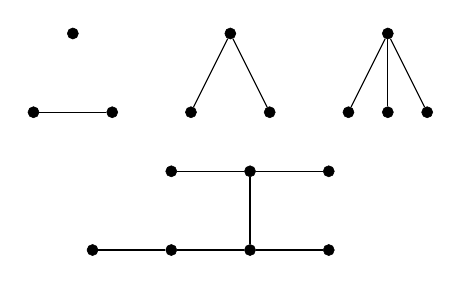
\begin{tikzpicture}[
	vertex/.style={ circle, draw, very thin, fill, inner sep=0pt, minimum size=4pt },
	vertexg/.style={ black!40!white, circle, draw, very thin, fill, inner sep=0pt, minimum size=4pt },
	vertexo/.style={ circle, draw, very thin, inner sep=0pt, minimum size=4pt }
]

\begin{scope}[xshift=0.5cm,yshift=1cm]
	\node[vertex] at (0,0) (v1) {};
\end{scope}

\node[vertex] at (0,0) (v2) {};
\node[vertex] at (1,0) (v3) {};
\draw (v3) to (v2);

\begin{scope}[xshift=2cm]
	\node[vertex] at (0,0) (v4) {};
	\node[vertex] at (0.5,1) (v5) {};
	\draw (v5) to (v4);
	\node[vertex] at (1,0) (v6) {};
	\draw (v6) to (v5);
\end{scope}

\begin{scope}[xshift=4cm]
	\node[vertex] at (0.5,1) (v7) {};
	\node[vertex] at (0,0) (v8) {};
	\draw (v8) to (v7);
	\node[vertex] at (0.5,0) (v9) {};
	\draw (v9) to (v7);
	\node[vertex] at (1,0) (v10) {};
	\draw (v10) to (v7);
\end{scope}

\begin{scope}[xshift=0.75cm,yshift=-1.75cm]
	\node[vertex] at (0,0) (v11) {};
	\node[vertex] at (1,0) (v12) {};
	\draw (v12) to (v11);
	\node[vertex] at (2,0) (v13) {};
	\draw (v13) to (v12);
	\node[vertex] at (2,1) (v14) {};
	\draw (v14) to (v13);
	\node[vertex] at (3,0) (v15) {};
	\draw (v15) to (v13);
	\node[vertex] at (3,1) (v16) {};
	\draw (v16) to (v14);
	\node[vertex] at (1,1) (v17) {};
	\draw (v17) to (v14);
\end{scope}

\end{tikzpicture}
